%%%%%%%%%%%%%%%%%%%%%%%%%%%%%%%%%%%%%%%%%%%%%%%%%%%%%%%%%%%%%%%%%%%%%%%%%
% This file is part of the LaTeX sources of the OMDoc 1.6 project descriptions
% Copyright (c) 2006 Erica Melis et al.
% This work is licensed by the Creative Commons Share-Alike license
% see http://creativecommons.org/licenses/by-sa/2.5/ for details
% The source original is at https://github.com/KWARC/OMDoc/doc/projects/activemath
%%%%%%%%%%%%%%%%%%%%%%%%%%%%%%%%%%%%%%%%%%%%%%%%%%%%%%%%%%%%%%%%%%%%%%%%%

\begin{omgroup}[id=activemath,short=ActiveMath,
  creators={melis,goguadse,alberto,frischauf,homik,libbrecht,cullrich}]
  {{\omdoc} in {\activemath}}

{\activemath} is a mature web-based intelligent learning environment for mathematics that
has been developed since 2000 at the University of Saarland and at the German Research
Institute of Artificial Intelligence (Intelligent Learning Environments Group headed by
Erica Melis). Its learning objects are encoded in an extension of {\omdoc}.

\begin{omgroup}{The {\activemath} System}

In addition to presenting pre-defined interactive materials, it adaptively generates
courses according to the learner's goals, learning scenarios, competencies, and
preferences. For this, {\twintoo{Tutorial}{Component}} requests
{\indextoo{learning}{object}s} \footnote{Following the classical definitions, learning
  objects are any resources that are used the learning activity. When in {\omdoc},
  learning objects considered are such as a \element{definition}, an \element{omtext} or
  an interactive exercise.}, related to the {\twintoo{learning}{goal}} to be retrieved
from several repositories.  The retrieval of object-IDs is realized by a mediator taking
into account structures and meta data of learning objects, and then the Tutorial Component
assembles them to a course skeleton depending on a {\twintoo{Learner}{Model}}.  For
details
see~\cite{Ullrich-TutorialPlanningYRT-AIED-2005,Ullrich-InstructionalOntology-ISWC-2004}.

In several stages a {\twintoo{Presentation}{Component}} fills and transforms this skeleton
to a material in the requested output format. In the interactive browser formats dummies
can represent Learning Objects that can be instantiated dynamically ---
depending on the learning progress or on requests by the user.

% learner model
This Learner Model stores the learning history, the user's profile and preferences, and a
set of beliefs that the systems holds about the cognitive and meta-cognitive competencies
and the motivational state of the learner. The domain model that underlies the structure
of the learner model is inferred from the content for that domain and its meta data
represented in the {\omdoc} source.
 
{\activemath} is internationalized and 'speaks' German, English, French, Spanish, Russian,
and Chinese by now. Its mathematical notation rendering can as well be adapted to
national' standards.
 
To realize a smooth and efficient cooperation of all components and in order to integrate
further internal and external services, {\activemath} has adopted a modular
service-oriented architecture displayed in Figure \ref{fig:LeAMarch}. It includes the
{\xmlrpc} web communication protocol for its simplicity and support. In addition, an event
framework enables the asynchronous messaging for any changes.

\begin{figure}[htp]
\begin{center}
  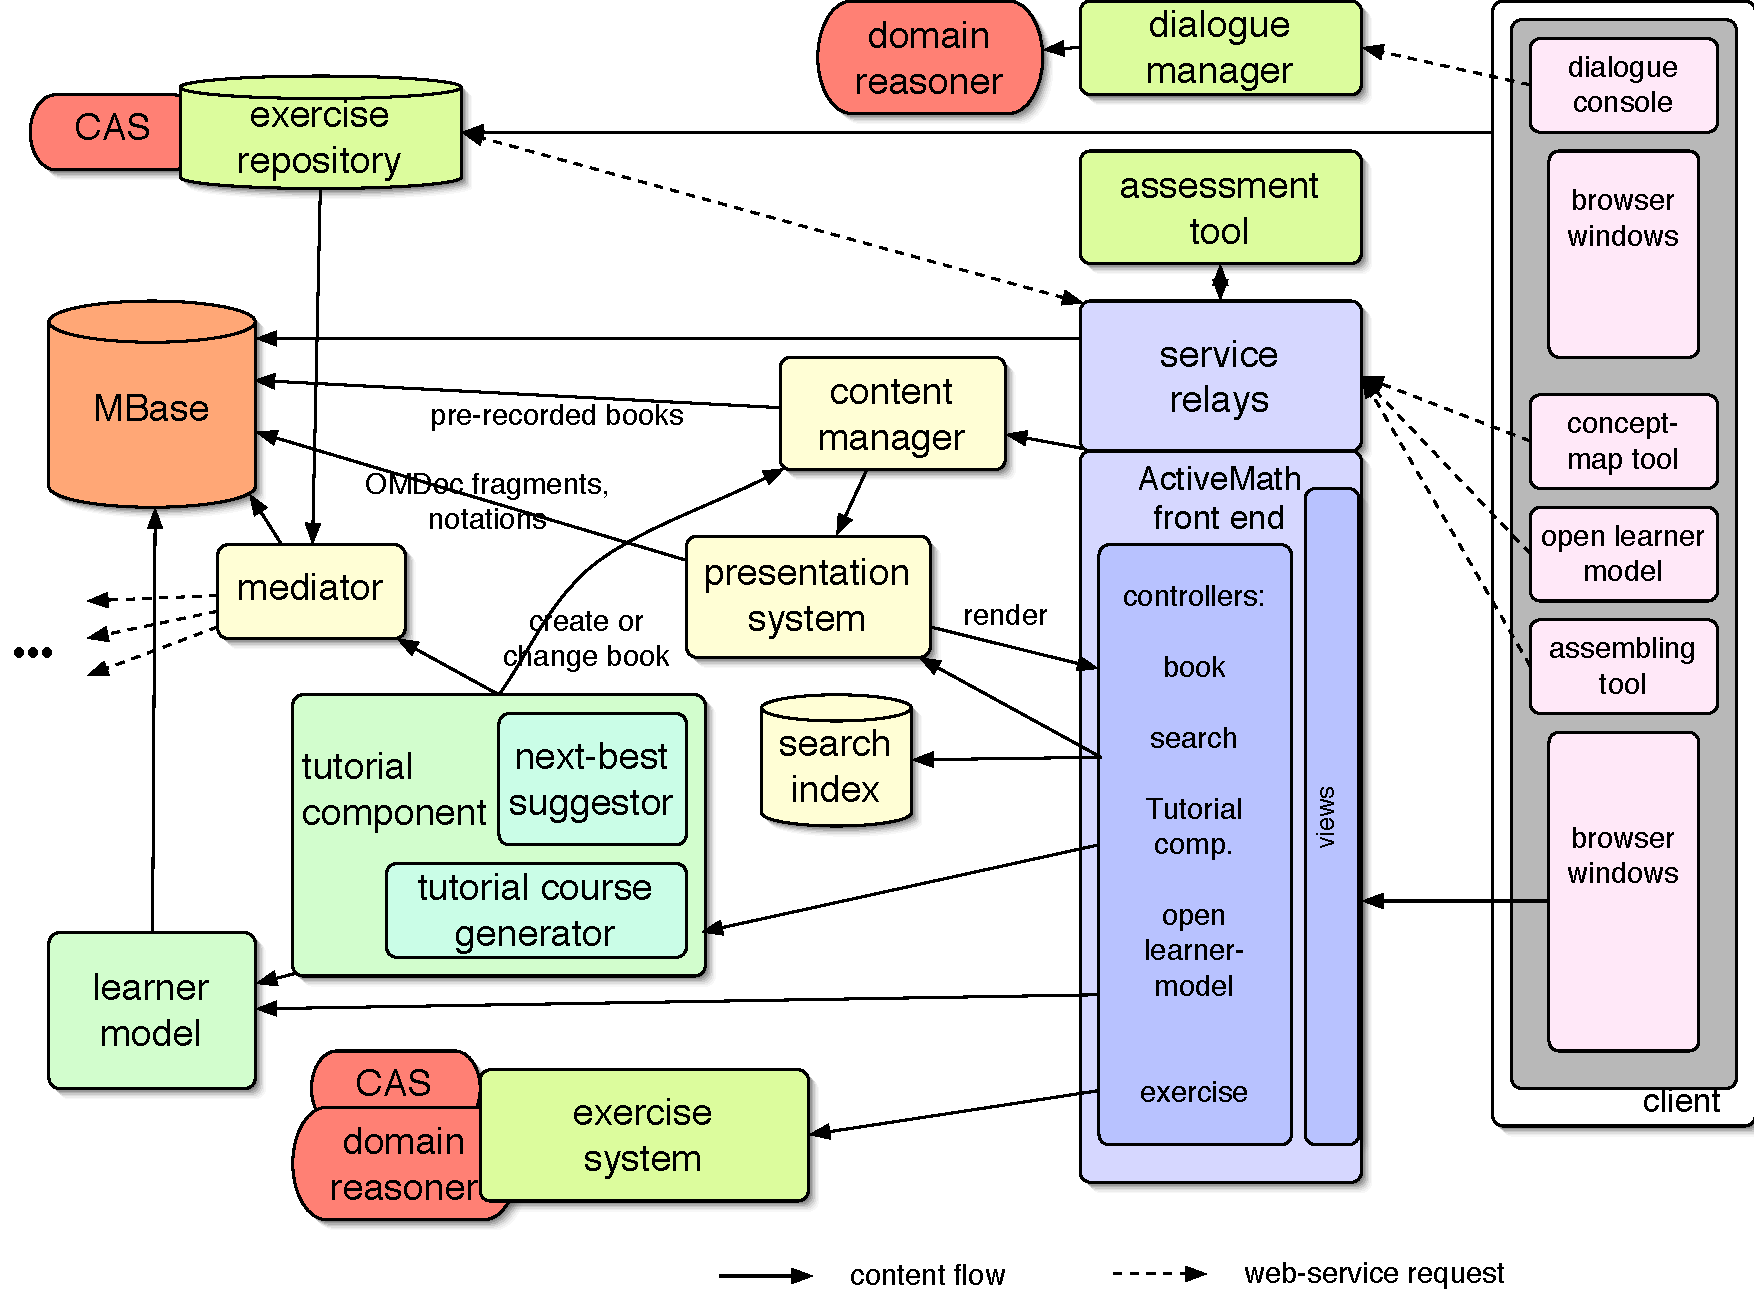
\includegraphics[width=11cm]{\projectsPath{activemath/diagrams/LeAMarchitecture}}
  \caption{The Components, Services and Information Flow in {\activemath}}
  \label{fig:LeAMarch}
\end{center}
\end{figure} 

A complex subsystem in its own right is {\activemath}'s exercise subsystem~\cite{icce05}
that plays interactive exercises, computes diagnoses and provides feedback to the learner
in a highly personalized way. It reports events to inform the other components about the
user`s actions.

In 2005, large educational contents exist in {\activemath}'s repositories for Fractions
(German), Differential Calculus (German, English, Spanish) at high school and first year
university level, operations research (Russian, English), Methods of Optimization
(Russian), Statistics and Probability Calculus (German), Mathef{\"u}hrerschein (German),
and a Calculus course from University of Westminster in London. 

\begin{omgroup}{{\activemath}'s  Service-Approach}
The encoding of content in {\omdoc} is an advantage for {\activemath}'s Web-service
approach. If available, the services -- including Web repositories -- can communicate more
semantic information than just meta data.  However, the interoperability of the content
encoding is only one side of the Semantic Web coin. Hence, the developments for
{\activemath} also include the reuse and interoperability of components and
tools~\cite{Melisetal-SemanticAware-BJET-2005}.

External services that are being connected currently are the {\scsys{Siette}} assessment
tool~\cite{Conejo-Siette-IJAIED-04} and one or more repository of interactive exercises
and interactive content.
\end{omgroup}
\end{omgroup}
\begin{omgroup}{{\omdoc} Extensions for {\activemath}}

The {\activemath} DTD extends the {\omdoc} DTD version 1.1 in several directions:
\begin{itemize}
\item new types of items such as \element{misconception}s, additional types of items such
  as types of exercises ({\tt{MCQ}}, {\tt{FIB}}, {\tt{map}}, {\tt{problem}}),
\item additional several relations with types such as {\tt{for}} or {\tt{prerequisite-of}},
\item other additional meta data such as {\element{difficulty}}, {\element{competency}}, or
  {\element{field}},
\item additional infrastructure as, e.g., in exercises, additional structure such as
  content packages~\cite{LeAMD6}.
\end{itemize}
The metadata and relation extensions are compliant with the Learning Metadata Standards
IEEE and IMS LOM~\cite{lom3_6,ims_lom}. Most of the extensions are
pedagogically/educationally motivated. Some details follow.

The educational metadata include {\tt{competency}} and {\tt{competencylevel}} that are used
for assessment, evaluation, and for adaptive suggestions of examples and exercises in
course generation.  As for competencies, {\activemath} supports Bloom's taxonomy of
learning goal levels~\cite{bloom56} and the more recent taxonomy from the Program for
International Student Assessment (PISA)~\cite{klieme04} and National Council of Teachers
of Mathematics (NCTM).

{\activemath} educational metadata include {\snippet{learning\_context}} which was in
first versions of LOM.  Metadata values, such as {\snippet{difficulty}},
{\snippet{abstract\-ness}}, and ``typical learning time'' have been annotated with the
corresponding learning context (allowing to say that an example is hard for an
undergraduate but not for a higher class).  The {\activemath} DTD introduced some
educational relation types which facilitate adaptive course generation and concept map
exercises, among others.

The {\omdoc} format has been refactored in {\activemath} in order to represent metadata in
a form that is separable from the representation of the knowledge item. For example, some
metadata represented in form of attributes of an item is moved inside the metadata
element. The purpose of such a separation is to facilitate the management of learning
materials in {\activemath}. Components such as Tutorial Component and Learner Model do not
deal with the content of the knowledge items but rather with their metadata only and hence
it is convenient to have a way to extract metadata records from the content.
 
For the internationalization each {\omdoc} item may have sub-elements in several languages
since {\activemath} does not translate learning objects on the fly.

{\activemath} extends the {\omdoc} {\element{example}} element. A detailed explanation can
be found in~\cite{Melisetal-FadedEx-ITS04-2004}.  In case of a worked-out example, the
micro-structure of this element is enriched with a solution that has a structure similar
to a proof in {\omdoc}.  It differs from the proof element since the solution might not
only prove a statement, but also calculate the value of some expression or explore the
properties of a particular structure (e.g. curve discussion).  This representation allows
for different presentations, and serves as a basis for the automatic generation of
exercises by fading some parts of the structure of a worked-out example
(see~\cite{Melisetal-FadedEx-ITS04-2004}).

The new exercise representation of {\activemath} was the basis for extending the Math QTI
standard~\cite{ENCS04}. Even though its origin can be traced to {\omdoc} originally not
much is left from the QUIZ representation of {\omdoc} which supports only very limited
types of exercises and did not have enough infrastructure.  The micro-structure of an
interactive exercise has to allow for different kinds of interactivity, checking the
correctness of the answer, providing feedback, etc.
%% An exercise in {\activemath} is represented as a graph of interactions 
%% between the exercise subsystem and a learner. It represents feedback and several types 
%% of hints.
This interaction graph can be automatically filled with information  
by the exercise subsystem components that can communicate with external systems in order 
to generate feedback to the user.

A description of {\activemath} language for exercises can be found in~\cite{icce05}.
\end{omgroup}

\begin{omgroup}{Usage of Semantic Representation in {\activemath}}
%%%%%%%%%%%%%%%%%%%%%%%%%%%%%%%%%%%%%%%%%%%%%%%%

The fact that the Tutorial Component employs metadata to search for appropriate learning
objects and assemble them has been sketched above. In addition, other tools and components
of {\activemath} make use of the semantics of {\openmath}, the {\activemath} metadata and
{\omdoc} more generally.

\begin{omgroup}{Computer Algebra Services}
Computer algebra system (CAS) --- currently {\scsys{Yacas}}~\cite{URL:Yacas},
{\scsys{Maxima}}~\cite{URL:Maxima}, and {\scsys{Wiris}}~\cite{URL:wiris-cas} --- are
integrated as external services. Via a broker, a CAS receives queries (partially Monet
queries) to evaluate {\openmath} expressions. This enables the exercise system to evaluate
user input, e.g., for numerical or semantic equivalence with a particular
expression. The service CAS has to translate in- and output via phrasebooks.
\end{omgroup}

\begin{omgroup}{Presentation Component}
The naive approach to rendering {\omdoc} documents would be to fetch the items from a data
base, assemble them (or parts of them) and then run several style-sheets on the resulting
sequence; Those style-sheets would depend on the requested output format (\html + Unicode,
\xhtml + {\mathml}, {\pdf} via {\LaTeX}, {\svg}, or slides), the target browser (we
support {\mozilla}, {\firefox}, Internet Explorer) and the personalization.

This approach turned out to be infeasible for complex, real-world applications. Therefore
{\activemath} includes a multi-stage presentation process as described
in~\cite{Ullrichetal-Presentation-ICALT04}. It has many advantages, among them a much
better performance and even better perceived performance through multiple caching, a clear
separation of different concerns which provides more flexibility for the various
adaptivity dimensions that {\activemath} supports, including selection of learning
objects, link annotations language, specific presentations of pages, exercises etc, and of
mathematical expressions, target output format, browser.

The final rendering maintains the references to mathematical symbols but renders them
invisible. This information can then be used by copy-and-paste and for tool tips that
indicate the name of a symbol on the page.

For an even more specialized presentation of mathematical notation which is often
requested by authors and users we developed a complex presentation tag representation and
an authoring facility for it~\cite{ManLib:apo05}. These special presentations are
integrated into the presentation process upon request.
\end{omgroup}

\begin{omgroup}{Copy and Paste}
The rendering includes an invisible reference to the unique identifier of mathematical
symbols and expressions. This provides a basis for copying the reference to an {\openmath}
expression, i.e., the semantics of the expression to a computer algebra system, to the
input editor (in dictionary and exercises), and into exercise blanks.
% For more details see~\cite{Paul!}. PL: no referenced yet!
The actual transfer mechanism is, because of security limitations and
because of resource management, a drag-and-drop operation which allows
immediate negotiation between the recipient and source. This allows
to transform to the appropriate encoding on demand.
Alternate encodings include {\openmath} with a restricted set of content-dictionaries, 
{\html} with embedded presentation and content {\mathml}.
Reference to {\omdoc} items and to pages of a book in {\activemath} are
exchangeable using the same paradigm.
\end{omgroup}
\begin{omgroup}{Interactive Concept Map Tool {\scsys{icmap}}}

{\scsys{icmap}} utilizes the {\omdoc} encoding and relations for generating feedback to
users' inputs~\cite{MelisKaergerHomikcmapDelphi05}. The tool visualizes (parts of) a
domain and relations between concepts and between concepts and satellites.
\end{omgroup}

\begin{omgroup}{Semantic Search}
{\activemath}'s search facility has been upgraded to enable not only approximate search
results but also to search semantically for ({\openmath}) mathematical expressions, for
certain types of learning objects and objects with particular metadata.
% For more details see~\cite{Paul!}: PL: have only an EU deliverable
The implementation of the search uses Jakarta Lucene with its high-performance
and easy deployment.
\end{omgroup}

\begin{omgroup}{{\omdoc}-Related Components and Tools of {\activemath}}
Many of the tools described above have not been sufficient for the purposes of a complex
and mature educational application such as {\activemath}.  Therefore, we had to improve
them or implement some from scratch. In particular, these include authoring tools (for
which improvement is still ongoing), transformation tools, validation tools, and
style sheets. Moreover, new tools have been developed or integrated into {\activemath},
e.g., an input editor that returns {\openmath}.

The conversion of {\omdoc} source to presentation code is done using {\xslt} style sheets. 
We started with the style sheets available in {\omdoc} repository and added to them the
{\activemath} linking schemata.
% which makes the {\activemath} web experience acceptable by learners.
These style sheets needed more polishing since they were too big and the management of
notations was not feasible.  Moreover, the {\TeX} oriented style sheets had to be
refurbished in order to work well with big documents.

Further tools have been realized within the authoring tools which are covered in
{\sref{jeditoqmath}}.
\end{omgroup}
\end{omgroup}
\end{omgroup}
%%% Local Variables: 
%%% mode: latex
%%% TeX-master: "../main"
%%% End: 


% LocalWords:  ActiveMath activemath Melis Goguadse Palomo Frischauf Homik GmbH
% LocalWords:  Libbrecht Carsten Ullrich Universit des Saarlandes omtext Ok MCQ
% LocalWords:  Mathef hrerschein Siette metadata IEEE IMS LOM competencylevel
% LocalWords:  NCTM QTI CAS Yacas Maxima Wiris activemath ness multi icmap
% LocalWords:  Lucene jeditoqmath activemath activemath activemath
